\documentclass{standalone}
\usepackage{tikz}
\usetikzlibrary{patterns, positioning}


\begin{document}
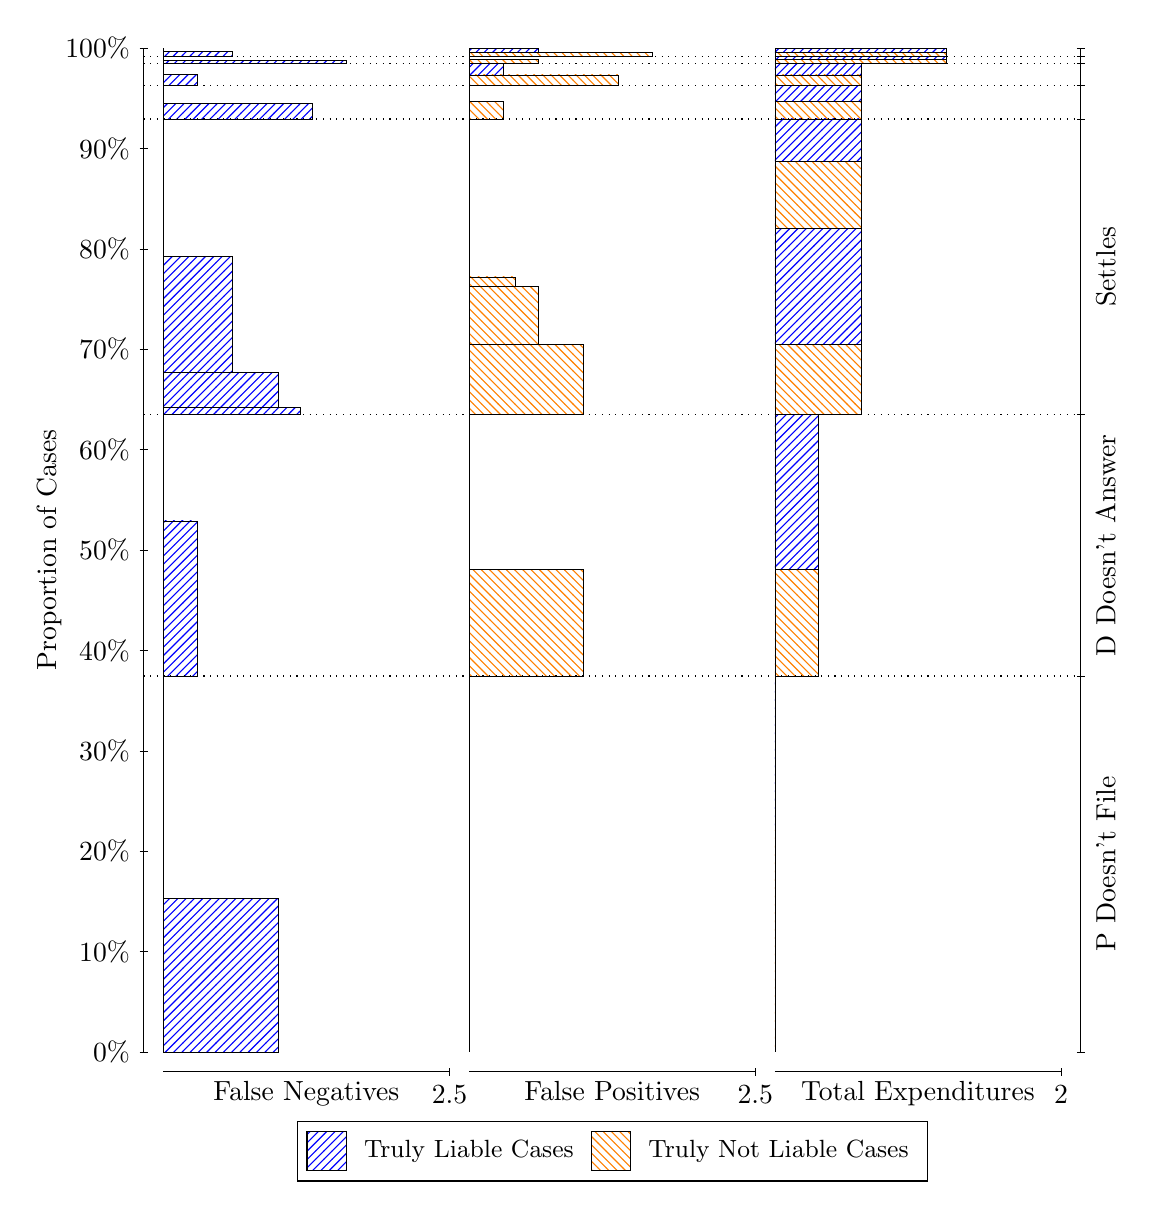
\begin{tikzpicture}
\draw[black, very thin] (1.5,1.75) -- (1.5,14.5);
\node[rotate=90, text=black, anchor=center] at (0.3, 8.125) {Proportion of Cases};
\draw[black, very thin] (1.45,1.75) -- (1.55,1.75);
\node[text=black, anchor=east] at (1.45, 1.75) {0\%};
\draw[black, very thin] (1.45,3.025) -- (1.55,3.025);
\node[text=black, anchor=east] at (1.45, 3.025) {10\%};
\draw[black, very thin] (1.45,4.3) -- (1.55,4.3);
\node[text=black, anchor=east] at (1.45, 4.3) {20\%};
\draw[black, very thin] (1.45,5.575) -- (1.55,5.575);
\node[text=black, anchor=east] at (1.45, 5.575) {30\%};
\draw[black, very thin] (1.45,6.85) -- (1.55,6.85);
\node[text=black, anchor=east] at (1.45, 6.85) {40\%};
\draw[black, very thin] (1.45,8.125) -- (1.55,8.125);
\node[text=black, anchor=east] at (1.45, 8.125) {50\%};
\draw[black, very thin] (1.45,9.4) -- (1.55,9.4);
\node[text=black, anchor=east] at (1.45, 9.4) {60\%};
\draw[black, very thin] (1.45,10.675) -- (1.55,10.675);
\node[text=black, anchor=east] at (1.45, 10.675) {70\%};
\draw[black, very thin] (1.45,11.95) -- (1.55,11.95);
\node[text=black, anchor=east] at (1.45, 11.95) {80\%};
\draw[black, very thin] (1.45,13.225) -- (1.55,13.225);
\node[text=black, anchor=east] at (1.45, 13.225) {90\%};
\draw[black, very thin] (1.45,14.5) -- (1.55,14.5);
\node[text=black, anchor=east] at (1.45, 14.5) {100\%};

\draw[black, very thin] (13.4,1.75) -- (13.4,14.5);
\draw[black, very thin] (13.35,1.75) -- (13.45,1.75);
\node[anchor=west] at (13.35, 1.75) {};
\draw[black, very thin] (13.35,6.525) -- (13.45,6.525);
\node[anchor=west] at (13.35, 6.525) {};
\draw[black, very thin] (13.35,9.8487) -- (13.45,9.8487);
\node[anchor=west] at (13.35, 9.8487) {};
\draw[black, very thin] (13.35,13.599) -- (13.45,13.599);
\node[anchor=west] at (13.35, 13.599) {};
\draw[black, very thin] (13.35,14.027) -- (13.45,14.027);
\node[anchor=west] at (13.35, 14.027) {};
\draw[black, very thin] (13.35,14.302) -- (13.45,14.302);
\node[anchor=west] at (13.35, 14.302) {};
\draw[black, very thin] (13.35,14.395) -- (13.45,14.395);
\node[anchor=west] at (13.35, 14.395) {};
\draw[black, very thin] (13.35,14.5) -- (13.45,14.5);
\node[anchor=west] at (13.35, 14.5) {};

\draw[black, very thin, pattern color=blue, pattern=north east lines] (1.75,1.75) rectangle (3.2033,3.7054);
\draw[black, very thin, pattern color=orange, pattern=north west lines] (1.75,3.7054) rectangle (1.75,6.525);
\draw[black, very thin, pattern color=blue, pattern=north east lines] (1.75,6.525) rectangle (2.186,8.4942);
\draw[black, very thin, pattern color=orange, pattern=north west lines] (1.75,8.4942) rectangle (1.75,9.8487);
\draw[black, very thin, pattern color=blue, pattern=north east lines] (1.75,9.8487) rectangle (3.494,9.9397);
\draw[black, very thin, pattern color=blue, pattern=north east lines] (1.75,9.9397) rectangle (3.2033,10.383);
\draw[black, very thin, pattern color=blue, pattern=north east lines] (1.75,10.383) rectangle (2.622,11.854);
\draw[black, very thin, pattern color=orange, pattern=north west lines] (1.75,11.854) rectangle (1.75,13.599);
\draw[black, very thin, pattern color=blue, pattern=north east lines] (1.75,13.599) rectangle (3.6393,13.801);
\draw[black, very thin, pattern color=orange, pattern=north west lines] (1.75,13.801) rectangle (1.75,14.027);
\draw[black, very thin, pattern color=blue, pattern=north east lines] (1.75,14.027) rectangle (2.186,14.17);
\draw[black, very thin, pattern color=orange, pattern=north west lines] (1.75,14.17) rectangle (1.75,14.302);
\draw[black, very thin, pattern color=blue, pattern=north east lines] (1.75,14.302) rectangle (4.0753,14.344);
\draw[black, very thin, pattern color=orange, pattern=north west lines] (1.75,14.344) rectangle (1.75,14.395);
\draw[black, very thin, pattern color=blue, pattern=north east lines] (1.75,14.395) rectangle (2.622,14.454);
\draw[black, very thin, pattern color=orange, pattern=north west lines] (1.75,14.454) rectangle (1.75,14.5);
\draw[black, very thin, pattern color=orange, pattern=north west lines] (5.6333,1.75) rectangle (5.6333,4.5697);
\draw[black, very thin, pattern color=blue, pattern=north east lines] (5.6333,4.5697) rectangle (5.6333,6.525);
\draw[black, very thin, pattern color=orange, pattern=north west lines] (5.6333,6.525) rectangle (7.0867,7.8795);
\draw[black, very thin, pattern color=blue, pattern=north east lines] (5.6333,7.8795) rectangle (5.6333,9.8487);
\draw[black, very thin, pattern color=orange, pattern=north west lines] (5.6333,9.8487) rectangle (7.0867,10.735);
\draw[black, very thin, pattern color=orange, pattern=north west lines] (5.6333,10.735) rectangle (6.5053,11.47);
\draw[black, very thin, pattern color=orange, pattern=north west lines] (5.6333,11.47) rectangle (6.2147,11.594);
\draw[black, very thin, pattern color=blue, pattern=north east lines] (5.6333,11.594) rectangle (5.6333,13.599);
\draw[black, very thin, pattern color=orange, pattern=north west lines] (5.6333,13.599) rectangle (6.0693,13.826);
\draw[black, very thin, pattern color=blue, pattern=north east lines] (5.6333,13.826) rectangle (5.6333,14.027);
\draw[black, very thin, pattern color=orange, pattern=north west lines] (5.6333,14.027) rectangle (7.5227,14.159);
\draw[black, very thin, pattern color=blue, pattern=north east lines] (5.6333,14.159) rectangle (6.0693,14.302);
\draw[black, very thin, pattern color=orange, pattern=north west lines] (5.6333,14.302) rectangle (6.5053,14.353);
\draw[black, very thin, pattern color=blue, pattern=north east lines] (5.6333,14.353) rectangle (5.6333,14.395);
\draw[black, very thin, pattern color=orange, pattern=north west lines] (5.6333,14.395) rectangle (7.9587,14.441);
\draw[black, very thin, pattern color=blue, pattern=north east lines] (5.6333,14.441) rectangle (6.5053,14.5);
\draw[black, very thin, pattern color=orange, pattern=north west lines] (9.5167,1.75) rectangle (9.5167,4.5697);
\draw[black, very thin, pattern color=blue, pattern=north east lines] (9.5167,4.5697) rectangle (9.5167,6.525);
\draw[black, very thin, pattern color=orange, pattern=north west lines] (9.5167,6.525) rectangle (10.062,7.8795);
\draw[black, very thin, pattern color=blue, pattern=north east lines] (9.5167,7.8795) rectangle (10.062,9.8487);
\draw[black, very thin, pattern color=orange, pattern=north west lines] (9.5167,9.8487) rectangle (10.607,10.735);
\draw[black, very thin, pattern color=blue, pattern=north east lines] (9.5167,10.735) rectangle (10.607,12.206);
\draw[black, very thin, pattern color=orange, pattern=north west lines] (9.5167,12.206) rectangle (10.607,13.065);
\draw[black, very thin, pattern color=blue, pattern=north east lines] (9.5167,13.065) rectangle (10.607,13.599);
\draw[black, very thin, pattern color=orange, pattern=north west lines] (9.5167,13.599) rectangle (10.607,13.826);
\draw[black, very thin, pattern color=blue, pattern=north east lines] (9.5167,13.826) rectangle (10.607,14.027);
\draw[black, very thin, pattern color=orange, pattern=north west lines] (9.5167,14.027) rectangle (10.607,14.159);
\draw[black, very thin, pattern color=blue, pattern=north east lines] (9.5167,14.159) rectangle (10.607,14.302);
\draw[black, very thin, pattern color=orange, pattern=north west lines] (9.5167,14.302) rectangle (11.697,14.353);
\draw[black, very thin, pattern color=blue, pattern=north east lines] (9.5167,14.353) rectangle (11.697,14.395);
\draw[black, very thin, pattern color=orange, pattern=north west lines] (9.5167,14.395) rectangle (11.697,14.441);
\draw[black, very thin, pattern color=blue, pattern=north east lines] (9.5167,14.441) rectangle (11.697,14.5);
\draw[black, dotted] (1.5,6.525) -- (13.4,6.525);
\draw[black, dotted] (1.5,9.8487) -- (13.4,9.8487);
\draw[black, dotted] (1.5,13.599) -- (13.4,13.599);
\draw[black, dotted] (1.5,14.027) -- (13.4,14.027);
\draw[black, dotted] (1.5,14.302) -- (13.4,14.302);
\draw[black, dotted] (1.5,14.395) -- (13.4,14.395);
\draw[black, very thin] (1.75,1.5) -- (5.3833,1.5);
\node[text=black, anchor=north] at (3.5667, 1.5) {False Negatives};
\draw[black, very thin] (5.3833,1.45) -- (5.3833,1.55);
\node[text=black, anchor=north] at (5.3833, 1.45) {2.5};

\draw[black, very thin] (5.6333,1.5) -- (9.2667,1.5);
\node[text=black, anchor=north] at (7.45, 1.5) {False Positives};
\draw[black, very thin] (9.2667,1.45) -- (9.2667,1.55);
\node[text=black, anchor=north] at (9.2667, 1.45) {2.5};

\draw[black, very thin] (9.5167,1.5) -- (13.15,1.5);
\node[text=black, anchor=north] at (11.333, 1.5) {Total Expenditures};
\draw[black, very thin] (13.15,1.45) -- (13.15,1.55);
\node[text=black, anchor=north] at (13.15, 1.45) {2};

\node[text=black, centered, rotate=90] at (13.72, 4.1375) {P Doesn't File};
\node[text=black, centered, rotate=90] at (13.72, 8.1869) {D Doesn't Answer};
\node[text=black, centered, rotate=90] at (13.72, 11.724) {Settles};





\draw (7.449999999999999,1.5) node[draw=none] (baseCoordinate) {};
\begin{scope}[align=center]
        \matrix[scale=0.5, draw=black, below=0.5cm of baseCoordinate, nodes={draw}, column sep=0.1cm]{
            \node[rectangle, draw, minimum width=0.5cm, minimum height=0.5cm, pattern color=blue, pattern=north east lines] {}; &
            \node[draw=none, font=\small, text=black] (B) {Truly Liable Cases}; &
            \node[rectangle, draw, minimum width=0.5cm, minimum height=0.5cm, pattern color=orange, pattern=north west lines] {}; &
            \node[draw=none, font=\small, text=black] (B) {Truly Not Liable Cases}; \\
            };
\end{scope}

\end{tikzpicture}
\end{document}